\subsection{Computer Vision Problems}
\begin{itemize}
    \item Image Classification
    \item Object Detection
    \item Neural Style Transfer
\end{itemize}


\subsection{Padding}
One modification that needs to be done in order to implement convolution in neural networks. 
For example, convolving a $3\times 3$ filter with a $6\times 6$ image results in a $4\times 4$ image. 

Generally, convolving a $f\times f$ filter with a $n\times n$ image yields a $n-f+1\times n-f+1$ image. 
Two downsides: 
\begin{itemize}
    \item Every time we convolve, the image shrinks. 
    \item Corner and edge pixels are only used once in computing the convolution. 
\end{itemize}

Padding helps resolve these issues: 
If the filter is $2k+1\times 2k+1$, pad the original image with $p = k$ pixel over each edge. As a result, the resulting image, the one 
that is fed into the convolution with the filter, will be $n+2p\times n+2p$. 

\subsection{Valid and Same Convolutions}
\begin{itemize}
    \item Valid: No padding, which means that convolving a $f\times f$ filter with a $n\times n$ image yields a $n-f+1\times n-f+1$ image.
    \item Same: The output size is the same as the input size (as explained above).  
    $$
    p = \frac{f-1}{2}
    $$
\end{itemize}

\subsection{Strided Convolutions}

Parameters of convolution: 
\begin{itemize}
    \item $n\times n$ image
    \item $f\times f$ filter
    \item $p$ padding
    \item $s$ stride
\end{itemize}

The size of the resulting image: 
$$
(\frac{n+2p-f}{s} + 1) \times (\frac{n+2p-f}{s} + 1)
$$

\subsection{Convolutions over Volumes}

We must use filters that are volumes themselves. For example, 
the convolution of a $6\times 6\times 3$ image with 
a $3\times 3\times 3$ filter yields a $4\times 4\times 1$ image. 
Note that the number of channels in the filter must be equal to 
the number of channels in the image. 
However, if we use multiple filters, for example, a filter that
detects vertical edges, and another filter that detects horizontal edges, 
the result will no longer be 2 dimensional. Generally: 
$$
(n\times n\times n_c) * (f\times f\times n_c) = ((n-f+1)\times (n-f+1)\times n_c^{'})
$$

Where $n_c^{'}$ is the number of filters. 

\begin{figure}[H]
    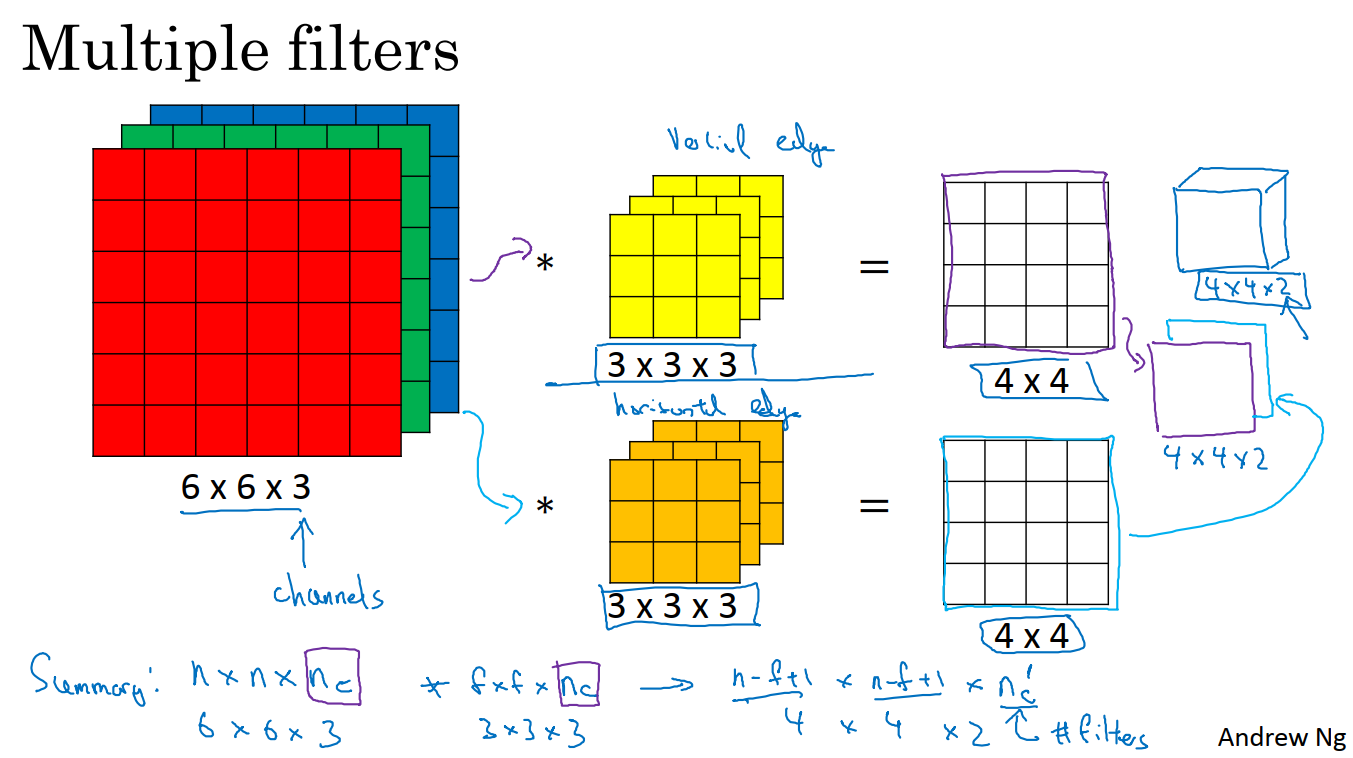
\includegraphics[scale=0.27]{images/volumes.png}
    \centering
\end{figure}

\subsection{One Layer of a CNN}
For each of convolution outputs, we are going to add a bias, 
and apply an activation function to the result of that addition. 
We have the same bias added to all pixels rather than 
having separate biases for each pixel. 

\textbf{Exercise:} If you have 10 $3\times 3\times 3$ filters, 
how many parameters does that layer have?

\begin{itemize}
    \item Filter Parameters: $10\times 3\times 3\times 3 = 270$
    \item One real number bias for each filter: $10\times 1 = 10$
\end{itemize}

So, a total of $280$ parameters. 

\textbf{Notation Summary:} If layer $l$ is a convolution layer: 


\begin{itemize}
    \item $f\lay{l}$: filter size
    \item $p\lay{l}$: padding
    \item $s\lay{l}$: stride
    \item $n\lay{l}_c$: number of filters = number of output channels
    \item $f\lay{l} \times f\lay{l} \times n\lay{l-1}_c$: each filter
    \item $n\lay{l-1}_H\times n\lay{l-1}_W\times n\lay{l-1}_c$: input
    \item $n\lay{l}_H\times n\lay{l}_W\times n\lay{l}_c$: output, where: 
    $$
    n\lay{l}_H = 1 + \frac{n\lay{l}_H + 2p\lay{l} - f\lay{l}}{s\lay{l}}
    $$
    $$
    n\lay{l}_W = 1 + \frac{n\lay{l}_W + 2p\lay{l} - f\lay{l}}{s\lay{l}}
    $$
    \item $a\lay{l}: n\lay{l}_H\times n\lay{l}_H\times n\lay{l}_c$: activations
    \item $A\lay{l}: m\times n\lay{l}_H\times n\lay{l}_H\times n\lay{l}_c$: vectorized activations
    \item $f\lay{l} \times f\lay{l} \times n\lay{l-1}_c\times n\lay{l}_c$: weights
    \item $1\times 1\times 1\times n\lay{l}_c$: biases
\end{itemize}

\subsection{Simple CNN Example}
\begin{itemize}
    \item Input: $39\times 39\times 3$
    \item Layer 1: 10 filters, each $3\times 3\times 3$ ($f=3$), no padding, stride $1$
    \item Output: $(1+\frac{39+0-3}{1}) \times (1+\frac{39+0-3}{1}) \times 10 = 37\times 37\times 10$
    \item Layer 2: 20 filters, each $5\times 5\times 10$ ($f=5$), no padding, stride $2$
    \item Output: $(1+\frac{37+0-5}{2}) \times (1+\frac{37+0-5}{2}) \times 20 = 17\times 17\times 20$
    \item Layer 3: 40 filters, each $5\times 5\times 40$ ($f=5$), no padding, stride $2$
    \item Output: $(1+\frac{17+0-5}{2}) \times (1+\frac{17+0-5}{2}) \times 40 = 7\times 7\times 40$
    \item Layer 4: Fully Connected...
\end{itemize} 

Layer Types in Conv Nets: 
\begin{itemize}
    \item Convolution (CONV)
    \item Pooling (POOL)
    \item Fully Connected (FC)
\end{itemize}

\subsection{Pooling Layers}

Pooling layers have no learnable parameters. Only $f$ and $s$ determine
how the pooling is done. Pooling is either max pooling or average pooling. 

\begin{figure}[H]
    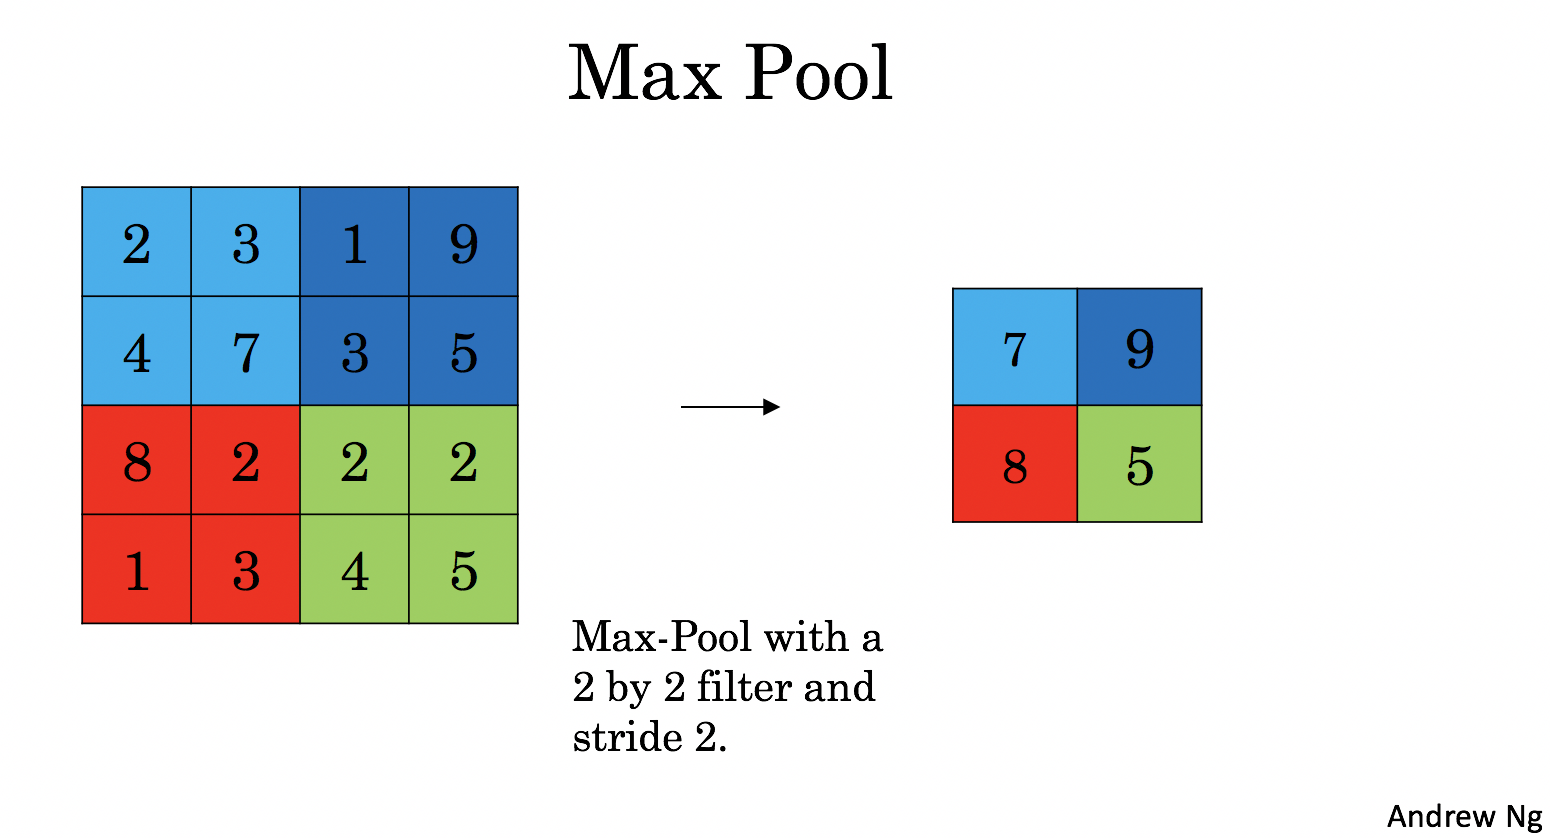
\includegraphics[scale=0.4]{images/maxpool.png}
    \centering
\end{figure}

The resulting image size is calculated just like how it was 
for convolutional layers: 
$$
(\frac{n+2p-f}{s} + 1) \times (\frac{n+2p-f}{s} + 1)
$$